\section{Theory}
\label{sec:theory}

This section is devoted to laying out a more formal description of the
theory presented in Section~\ref{sec:intro}. While the particles and
their properties tabulated in Figure~\ref{fig:sm} summarize the important
players in the study of elementary particles, an understanding of the
mathematical ideas behind the Standard Model's construction are essential in grasping
the importance of this measurement. This paper is focused on the measurement
of \HToZg at the LHC; therefore, a rigorous development of this ideas is forgone. 
For this see Halzen and Martin~\cite{QuarksLeptons}.

% Section~\ref{subsec:qed} gives a brief
% introduction to Gauge Theory and Quantum Field Theory through the simplest
% theory contained in the Standard Model: Quantum Electrodynamics (QED).
% Afterward the Higgs Mechanism is explained in Section~\ref{subsec:higgsmec}
% and finally the production processes studied in this measurement are
% given in Section~\ref{subsec:prodproc}.


\subsection{The Role of Symmetry in Particle Physics}
\label{subsec:symmetry}

An important principle motivating the mathematical structure of modern physical 
theories is the notion of symmetry. On a macroscopic scale one can study
the interactions of objects by holding them at various
distances apart and measuring the force between them. That is how Coulomb derived
the famous inverse square law describing electric repulsion and attraction that
now bears his name. On the smallest scales this empirical data is no longer
available, so that a new paradigm is need to understand how these interactions
come about. 

A beautiful solution was brought to light by the brilliant 
mathematician and physicist Emmy Noether who showed that every symmetry in
nature leads to a conserved quantity, a value that does not change over time.
A familiar application of this connection is found in Newton's third law:
For every action there is an equal and opposite reaction. From this balancing of
forces one can derive a conserved quantity associated with the system's 
motion, namely momentum. The importance of Noether's approach using symmetries
is that it allows the physicist to turn this reasoning around. One can postulate
the existence of a symmetry of nature, in this case the invariance of the laws
of physics under translations in space, which leads to a conserved quantity (momentum)
that results in experimentally testable predictions (Newton's third law).

While quantities such as momentum are familiar at the macroscopic level, 
it turns out that similar symmetries exist at subatomic distances
known as internal symmetries. One of the first examples of these symmetries
known as isospin was put forth by Werner Heisenberg in 1932 
to explain the approximate symmetry between
the newly discovered neutron with its partner in the atomic nucleus, the proton.
This symmetry says that according to the strong interaction that holds
the nucleus together the neutron and proton are reflections of each other,
i.e. the exchange proton $\leftrightarrow$ neutron does not affect the
physics of the strong force. More importantly this symmetry predicts that the
scattering rates of the interactions
\begin{align*}
    & p + p \rightarrow \pi^+ + d \\
    & \underbrace{p}_{\text{proton}} + \underbrace{n}_{\text{nuetron}} \rightarrow \underbrace{\pi^0}_{\text{pion}} + \underbrace{d}_{\text{deuteron}}
\end{align*}
should be equal. The experimental verification of this prediction convinced
physicists that these internal symmetries can be used to study and predict
how particles interact at the smallest length scales.

Physicists now use similar internal symmetries known as gauge symmetries to
describe the fundamental particles and their interactions. These gauge symmetries
are mathematical constructs similar to isospin that predict force carrying 
particles that mediate interactions in a way that can be used to calculate
various measurable quantities. The current gauge-theory formulation which describes
much of the phenomena found in nature is known as the Standard Model.

\subsection{The Standard Model}
\label{subsec:StandardModel}
A picture of the Standard Model of particle physics is best obtained
by moving away from the abstract gauge-theory formulation and instead considering
the predictive outcomes of the theory. The Standard Model provides physicists with
the current answer to the question of what the world is made of and is displayed
in Figure~\ref{fig:sm}. This table is reminiscent
of the periodic table developed by chemists to explain the various atoms
found in nature. Similar to the periodic table, the placement of particles in 
Figure~\ref{fig:sm} tells us something about the structure of these particles and
how they interact with each other. Some of these properties are labeled on
the figure including the particle's mass, charge, and 
spin\footnote{Spin is an internal quantum number of a particle which manifests 
itself as a particles intrinsic angular momentum.}.

\begin{figure}[htbp]
    \centering
    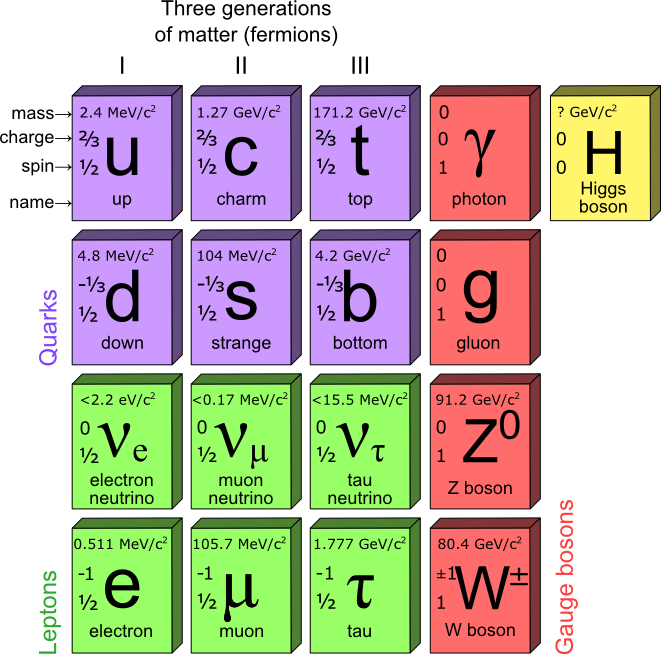
\includegraphics[scale=0.4, angle=0]{./figures/StandardModelPNG}
    \caption{A table summarizing the particles described by the
    Standard Model of particle physics. The Standard Model encompasses
    three generations of quarks and leptons as well as four force carrying
    bosons.}
    \label{fig:sm}
\end{figure}

A surprising property of the Standard Model is that it consists
of only 16 different particles. The first three columns consist of particles
that make up everyday matter known as fermions. A fermion is any particle that
has spin 1/2. 
For example, the first column contains two particles shown in purple known as
the up and down quarks, which are the building blocks of the familiar nucleons, 
i.e. the proton and the neutron. 
In addition, the second two particles marked in green
are the electron neutrino, which is produced abundantly in nuclear beta decay
($n \to p + e^- + \bar{\nu}_e$), as well as one of the most familiar fundamental
particles, the electron. In fact the atoms of the periodic table result when
the electron binds with the nucleons made of up and down quarks to form atoms. 
The Standard Model contains
three copies of this column structure composed of ever heavier particles.

The fundamental fermions are further divided into two types: quarks and leptons.
These forms of matter are separated by the various `charges' they carry. Quarks
(colored in purple in Figure~\ref{fig:sm})
carry both electric and color charge, so that they are the only particles that
interact via the strong force. 
On the other hand, leptons (colored in green in Figure~\ref{fig:sm}) 
do not carry color charge, so they do not interact with the strong force.
An important observation is that the ability of the quarks to interact via the
strong force allows them to overcome their electromagnetic repulsion and bind
together to form hadrons, particles composed of quarks. The proton and nuetron
are both examples of hadrons. Hadrons are further classified by the number
of constituent quarks that make them up. Baryons are made of three quarks while
mesons contain a quark and an anti-quark 
The proton, which is made of $uud$ quarks, is a baryon and
the $\pi^+$ is an example of a meson made up of $u\bar d$ quarks.
The various particle classifications used in particle physics are summarized in
\refF{fig:partclass}.

\begin{figure}[htbp]
    \centering
    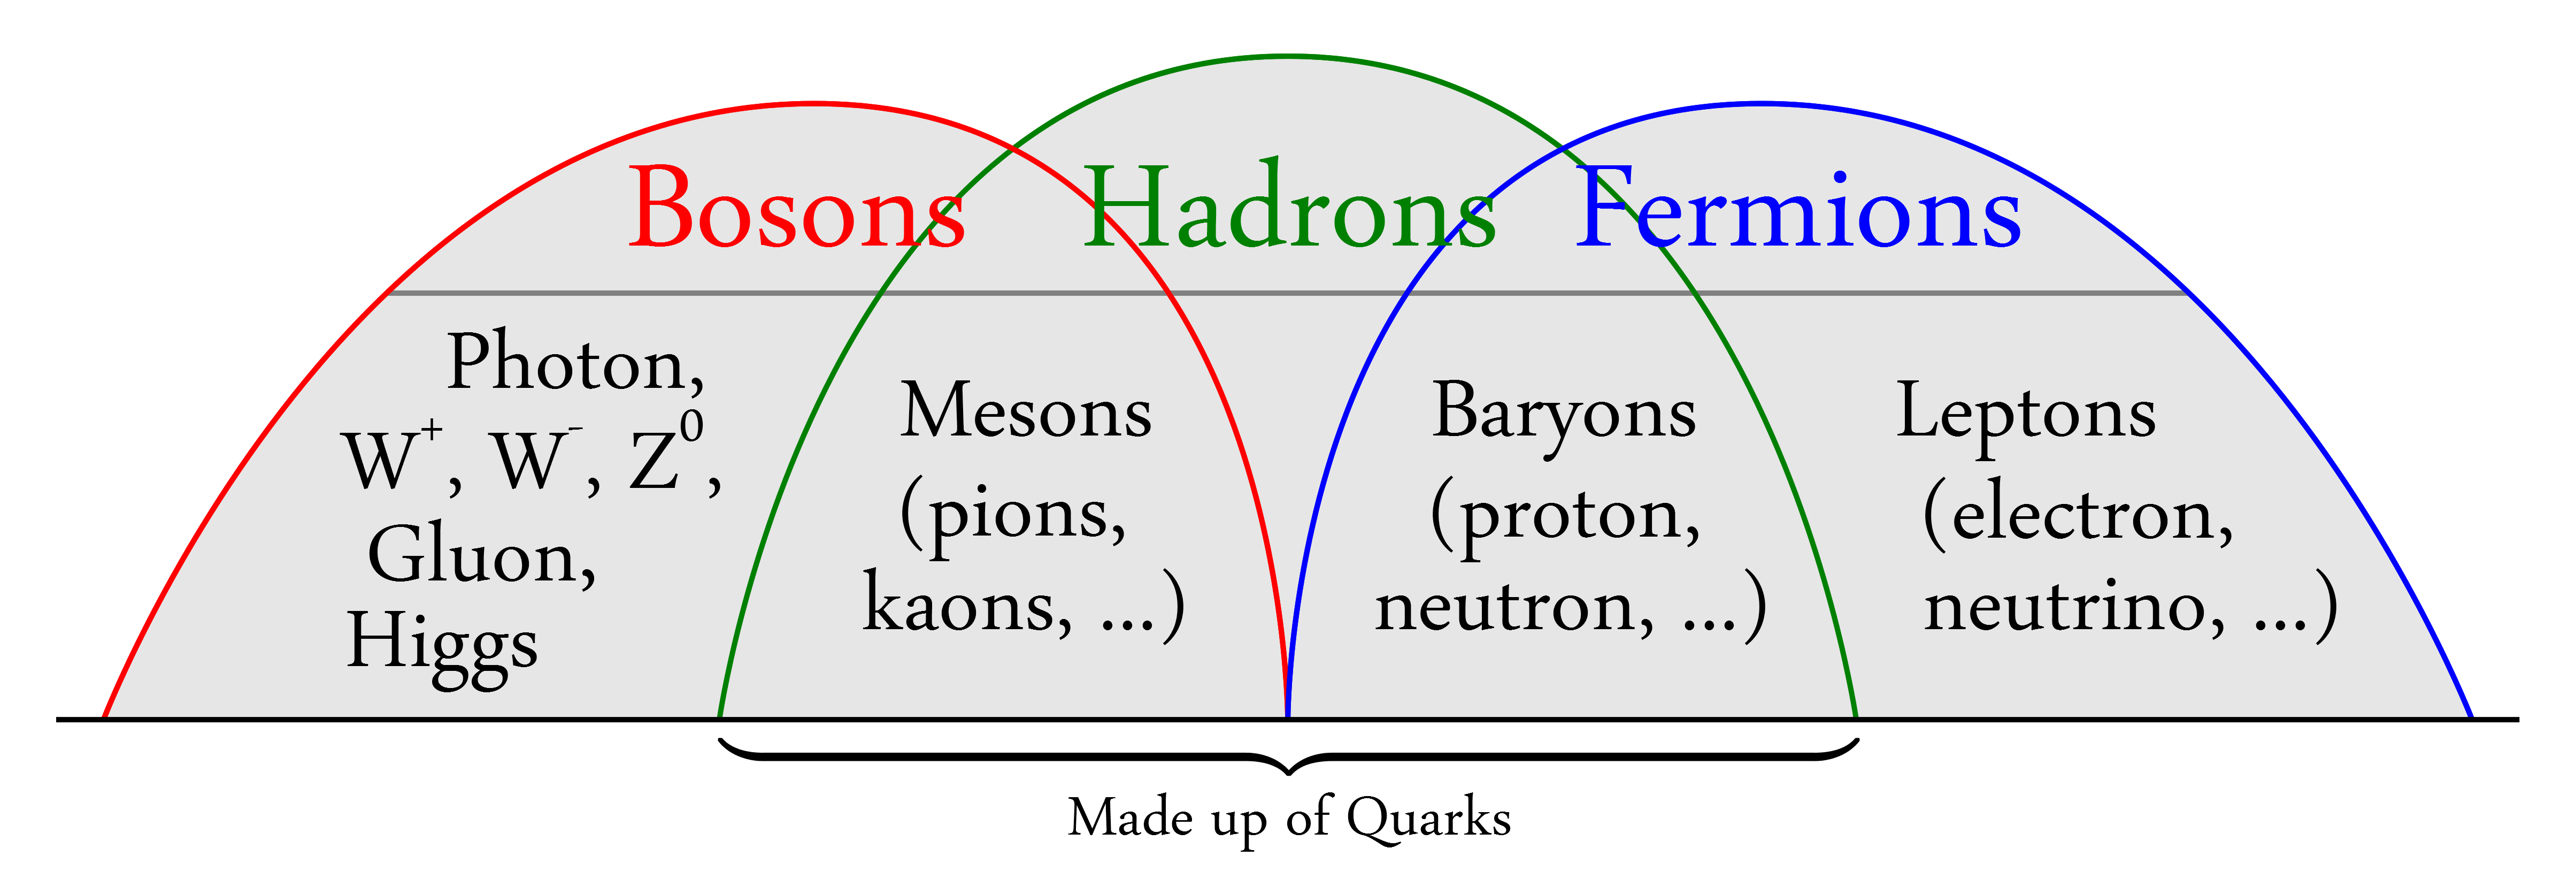
\includegraphics[scale=0.08, angle=0]{./figures/Bosons-Hadrons-Fermions}
    \caption{The different classifications of particles used in particle physics. Notice that hadrons are composed of both mesons and baryons, which are made up of quarks.
    The leptons are considered fermions because they have spin 1/2. The force carrying particles are bosons.}
    \label{fig:partclass}
\end{figure}

Finally there are four force carrying particles highlighted in red associated
with the gauge symmetries of the Standard Model. Mathematically, the gauge 
symmetry of the Standard Model is labeled as 
\[
\underbrace{\text{SU}(3)}_{\text{Strong Force}} \times \underbrace{\text{SU}(2) \times \text{U}(1)}_{\text{Electroweak Force}}.
\]
What this means is that each gauge symmetry is associated with particles.
These particles are known as gauge bosons and are responsible for mediating three 
out of the four fundamental forces in nature: the electromagnetic, strong, and 
weak interactions. As of now, theorists have been unable to incorporate the 
gravitational force, a pervasive component of the macroscopic world,
into the current gauge-theory of particle physics.
The SU(3) gauge symmetry describes the strong force, which
is mediated by the massless gluon. This force is responsible for binding
quarks together to form protons and neutrons. The weak interaction is
contained in the SU(2) gauge symmetry and is transmitted by the massive \WBosons
and \ZBoson bosons. The weak force is responsible for radioactive decays. The
last symmetry of the Standard Model, U(1), describes the familiar electromagnetic
interaction and is carried by the massless photon. The interaction of the force
carrying bosons with the Standard Model particles is graphically represented in 
\refF{fig:interactions}.

\begin{figure}[htbp]
    \centering
    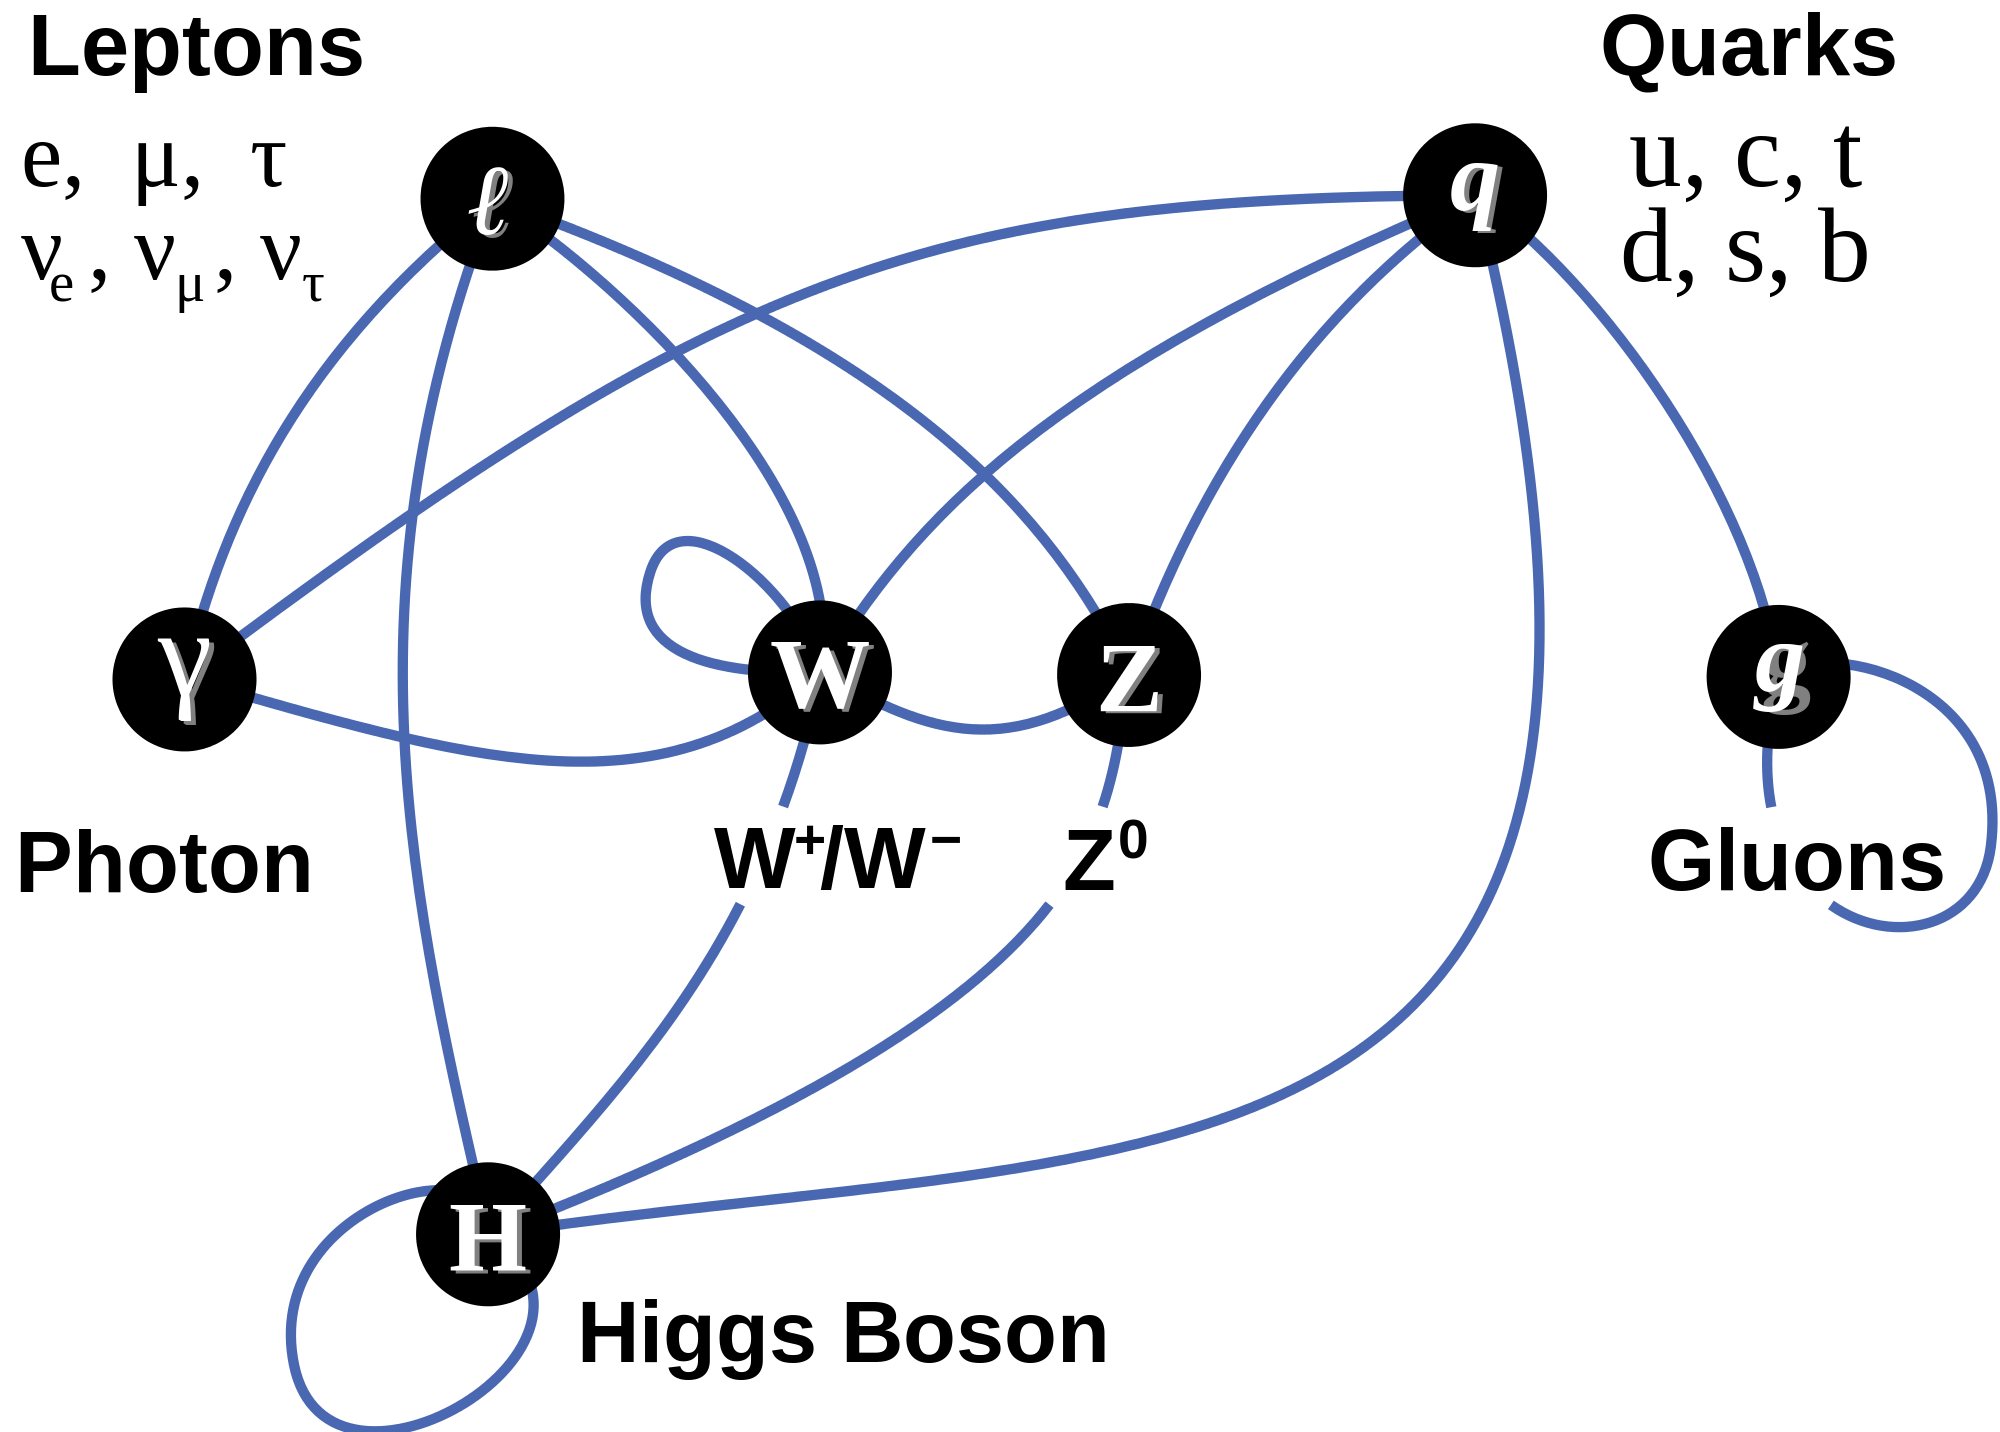
\includegraphics[scale=0.1, angle=0]{./figures/Elementary_particle_interactions}
    \caption{A graphical summary of the various interactions between particles 
    predicted by the Standard Model. 
    Notice that the leptons do not couple to the gluons, while
    the quarks couple to gluons as well as the electroweak force carriers.}
    \label{fig:interactions}
\end{figure}

The Standard Model together with Einstein's theory of gravity describes almost
all known phenomena from the largest scales to the smallest scales. Despite
its ability to precisely predict a large variety of experimental results, the
Standard Model does not account for the complete picture. Although not exhaustive
the following list contains a few inadequacies of the Standard Model:
1) It does not attempt to explain gravitation. As of yet a quantum theory of
gravity remains unknown.
2) The model contains 19 numerical constants whose values are not predicted
by the theory.
3) The Standard Model has no mechanism to explain the presence of the measured
missing mass and energy in the universe, the so called dark matter and dark energy 
problem. Despite these shortcomings, the gauge symmetries of the Standard Model 
remain a very powerful predictive tool responsible for explaining much of
what we know about the subatomic world.


\subsection{The Higgs Mechanism}
\label{subsec:higgsmec}
However, there is a problem with this extensive use of gauge symmetry.
While the Standard Model formulated in this way
is able to correctly describe much of what is seen by experiment, it
incorrectly predicts that the weak force is a long range force. There is
nothing inherently wrong with this outcome; however, observations show 
that the weak nuclear force has a range of roughly $10^{-18}$ meters, roughly
this size of a nucleus. The reason for this discrepancy is that the
\WBosons and \ZBoson bosons are
not massless particles, but have a mass of roughly 80 and 90 GeV respectively
\footnote{A crude way to see this is to consider Heisenberg's Uncertainty
principle. The range of the weak force is roughly
\[
    R_{\text{weak}} = c\Delta t \le \frac{\hbar c}{\Delta E} = \frac{\hbar c}{2 M_{Z}} \approx 10^{-18}\, \text{m}
\]
where $M_{Z}$ is the mass of the \ZBoson boson.
}.
In fact, these internal gauge symmetries predict that the other fundamental
particles, such as the electron, are massless.
In order to solve this apparent predicament one needs to introduce a mechanism
that keeps the Standard Model's equations symmetric under the SU(3) $\times$
SU(2) $\times$ U(1) gauge symmetries since this theory is correct in
almost all regards, but gives the fundamental particles mass.
This is accomplished by the Higgs mechanism, which combines two theoretical ideas
known as spontaneous symmetry breaking and local gauge invariance to introduce
mass into the theory.

Spontaneous symmetry breaking provides the solution to the first problem:
the equations governing a theory's behavior are symmetric, but the lowest
energy and most probable state, i.e. ground state, is not. Cases of this idea
are not just confined to subatomic physics, but are commonly found on a
macroscopic scale. For example consider holding a ruler between your index
finger and your thumb and squeezing down on the top of the ruler 
as shown in \refF{fig:ruler}. This system
is completely symmetric about the axis of the ruler: the force is along the $z$-axis
and the $z$-axis is the ruler's axis of symmetry. However, when the force
becomes strong enough, the ruler will snap into a left or right configuration since
both are ground states for the system. This choice of ground state breaks the
left-right symmetry of the physical system. A more mathematical presentation
of this symmetry breaking is presented in \refF{fig:rulerpotential}. The potential
of the system is plotted as a function of the displacement $y$ of the center of 
the ruler. The potential is symmetric about the origin $y = 0$; however,
the system will come to rest at one of the two minimum ground states at $y = 1$ or -1.
This choice of ground state breaks the symmetry of the potential, although
the potential remains symmetric.

\begin{figure}[htbp]
   \centering 

    \begin{subfigure}[b]{0.45\textwidth}
        \centering
        \includegraphics[scale=0.4, angle=0]{./figures/RulerAxes}
        \caption{}
        \label{fig:ruler}
    \end{subfigure}
    \quad 
    \begin{subfigure}[b]{0.45\textwidth}
        \centering
        \includegraphics[scale=0.8, angle=0]{./figures/RulerPotential}
        \caption{}
        \label{fig:rulerpotential}
    \end{subfigure}

    \caption{An example of spontaneous symmetry breaking in a 1-dimensional system
    is depicted in (a).
    The buckling of a ruler when a force is applied parallel to its axis of
    symmetry results in an asymmetric ground state although the original system
    is symmetric about the $z$-axis. This idea expressed in terms of the system's 
    potential is shown in (b).}
    \label{fig:spontaneous}
\end{figure}

When this idea of spontaneous symmetry breaking is combined with the local gauge
invariant description of the Standard Model, the familiar masses of the fundamental
particles are produced. The Higgs mechanism postulates a new field, the Higgs field,
that permeates throughout space. This field is shown in \refF{fig:higgspotential} and
the different energy states correspond to any point on the surface of this
`hat' potential. The point on the top of the hat, indicated by a blue ball
in \refF{fig:higgspotential}, corresponds to the symmetric ground state. This
means that the potential looks the same as it is rotated about an
axis going down through this point\footnote{This 1-dimensional rotational
symmetry is actually what is meant by a theory being U(1) invariant.}. However,
this ground state is not the lowest energy state. The minimum energy states
occur on the circle at the bottom of this hat. Intuitively, nature
chooses a point randomly at the bottom to call the ground state.
This state -- in the exact same way as the example of the ruler -- is no longer
symmetric under rotations, it is an asymmetric ground state.

\begin{figure}[htbp]
    \centering
    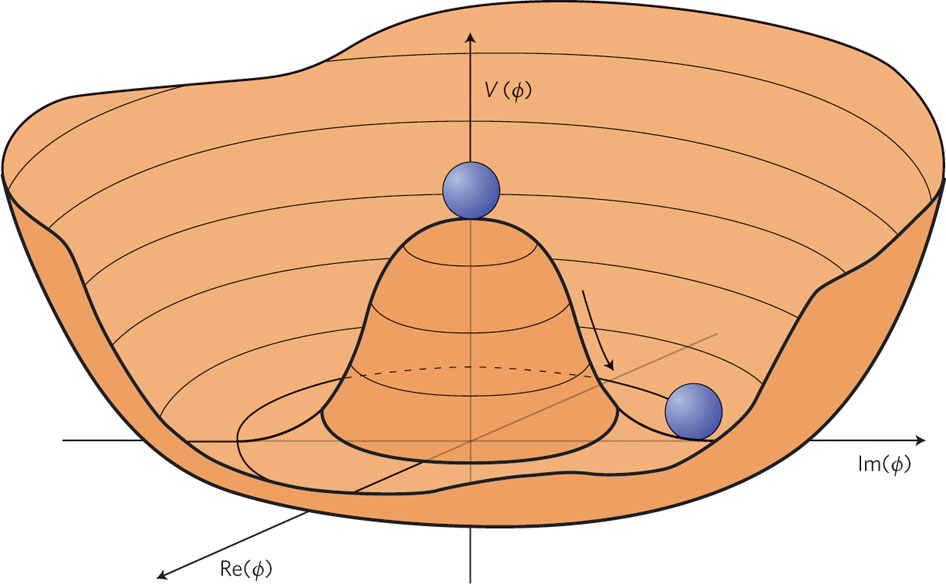
\includegraphics[scale=0.35, angle=0]{./figures/HiggsPotential}
    \caption{The vacuum -- that is, the lowest-energy state -- is described by
    a random chosen point around the bottom of the hat. In a global symmetry,
    movements around the bottom of the hat correspond to a massless, spin-zero,
    Goldstone boson. In the case of a local gauge symmetry this boson combines
    with the massless spin-one boson to yield a massive spin-one particle. The
    Higgs boson is a massive spin-zero particle corresponding to quantum
    fluctuations in the radial direction, oscillating between the center and
    the side of the hat in the direction of the arrow~\cite{HiggsPic}.}
    \label{fig:higgspotential}
\end{figure}

The physical reality described in terms of particles and their masses comes 
by interpreting this field quantum mechanically.
In quantum mechanics for every field there is a
corresponding particle associated with fluctuations about the field's ground
state. In the case of the Higg's field there are two possible ways to fluctuate
about the asymmetric ground state: around the smooth surface of the circular well
or inward about the curved bowl of the hat. This gives rise to two distinct 
particles. The fluctuations around the bottom of the well give rise to a particle 
known as a Goldstone boson that remains massless because there is no resistance
to its movement around the well. However, this extra particle is exactly what
is needed to cure the problem of missing mass. The Goldstone boson injects
a needed extra degree of freedom into the theory
that can be absorbed by the \WBosons and \ZBoson
bosons to give them mass and make the weak force short ranged. In addition, 
the Higgs field allows for
another massive particle corresponding to fluctuations in the radial
direction: the Higgs boson. In summary, the Higg's mechanism postulates a new field
radiating throughout space that couples to various particles giving them mass
and predicts that a new particle known as the Higgs boson should be observable
in nature.


\subsection{Production Process}
\label{subsec:prodproc}

\begin{figure}[!htbp]
  \begin{center}
  {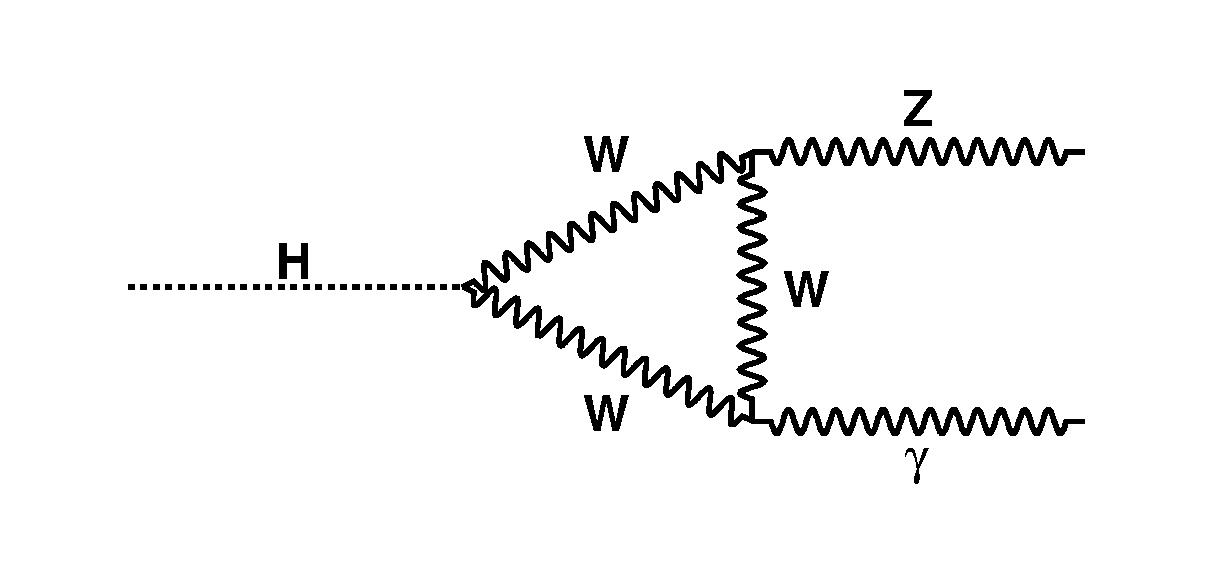
\includegraphics[width=2in]{figures/loop1}}
  {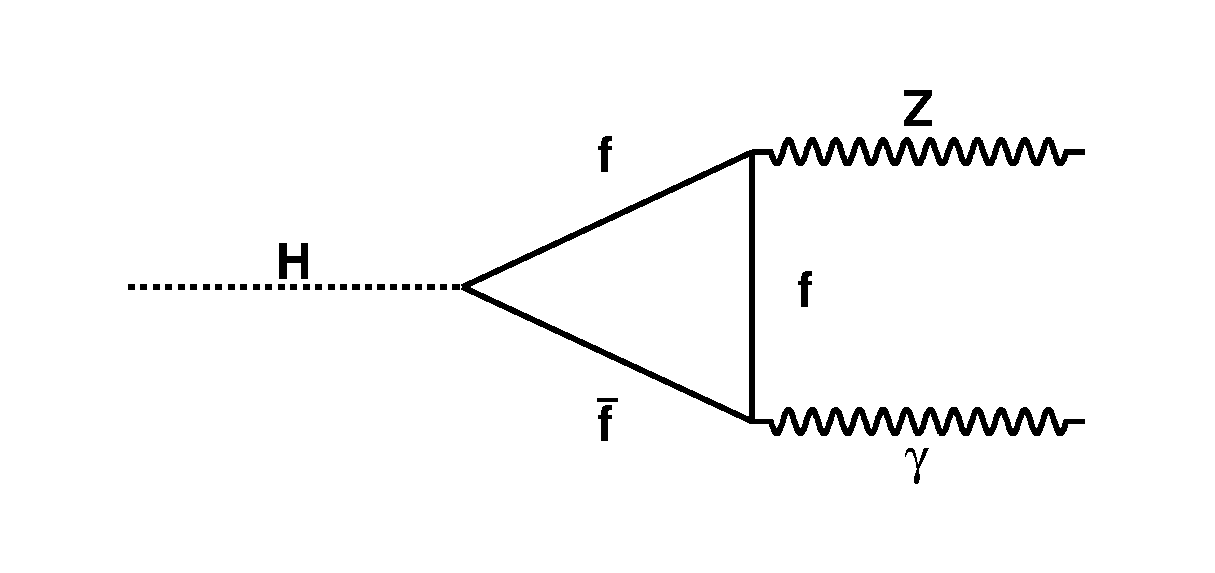
\includegraphics[width=2in]{figures/loop2}}
  {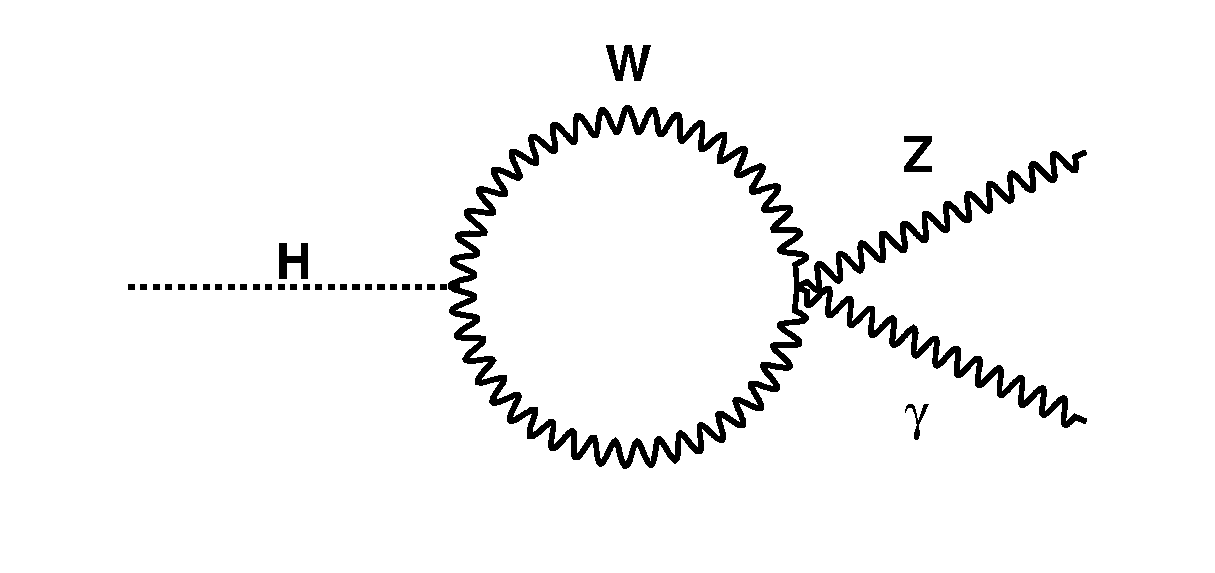
\includegraphics[width=2in]{figures/loop3}}
  \caption{Leading Feynman diagrams for the $H\rightarrow Z\gamma$
    decay in the Standard Model. Note that in the case of the fermion
    loop, top quarks dominate.} 
  \label{fig:feynman}
  \end{center}
\end{figure}
